\documentclass{article}
\usepackage[utf8]{inputenc}
\usepackage[spanish]{babel}
\usepackage{amsmath}
\usepackage{paracol} % Paquete para manejo de columnas
\usepackage{lipsum}
\usepackage{graphicx} % Paquete para inserción de imágenes
\usepackage{xcolor}

\graphicspath{{../images/}} % Ruta de almacenamiento de las imágenes

\title{Título del artículo}
\author{Johan Sebastian Mastropiero}
\date{\today}

\begin{document}
	\maketitle
	\begin{abstract}
		\lipsum[1]
	\end{abstract}

	\columnratio{.6} % Modifica el ancho de la columna 1 (primera a la izquierda)
	\begin{paracol}{2}[\section{Título muy largo para la primera sección}]
		\subsection{Columnas sincronizadas}
		\lipsum[3]
		\switchcolumn % Cambio de columna
		\lipsum[2]
		\switchcolumn* % Columna sincronizada
		Columna sincronizada
		\[
			\frac{d}{dx}(\sinh ^{-1}x) = \frac{1}{\sqrt{1 + x^2}}
		\]
		\switchcolumn
		\lipsum[2]
		\switchcolumn*
		\lipsum[1]
		\switchcolumn
		\lipsum[2]
	\end{paracol}

	\section{De vuelta a la distribución de una sola columna}
		\lipsum[7-8]
		\columnratio{.4}
		\columncolor{red} % cambia el color del texto de toda la columna
		\begin{paracol}{2}
			\lipsum[5]
			\switchcolumn
			\begin{figure}[ht] % Inserta una figura
				\centering
				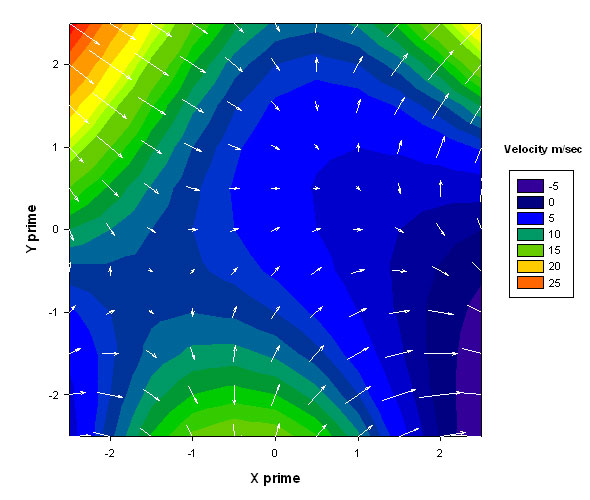
\includegraphics[scale=.35]{2Dvectorplot.jpg}
				\caption{Flotantes en paracol}
			\end{figure}
		\end{paracol}
\end{document}
